\clearpage
\section{Data, cohorts, and parcellations}\label{sec:ukb-data}
%%%%%

\info[inline]{Paragraph: Broad introduction of data and phenotyping.}
All data and cohorts are taken from the UK Biobank, a large population study data bank.
A four-by-two analysis is performed, studying four depression phenotypes (that define four sets of cohorts) and two levels of brain abstractions.
These four phenotypes are: (inpatient) diagnosed lifetime occurrence of \gls{mdd}, self-reported depression lifetime occurrence, self-reported depressive state (at the time of the brain scan), and depression genetic risk as measured by \gls{prs}.
The two abstractions (i.e.~parcellations) are as a collection of individual (relevant) brain \glspl{roi} and as a superposition of (relevant) \glspl{fn}.
Carefully slicing cohorts in several ways may yield insights beyond a single study.

%%
\subsection{Data overview}
%%

\info[inline]{Paragraph: Introduce UK Biobank.}
The UK Biobank is a large, actively growing, and publicly available data biobank of 502,486 unique individuals located across the United Kingdom, recruited voluntarily from the general populace~\parencite{Collins2012, Allen2014b}.
Despite some `healthy volunteer' biases that affect how representative this data is of the entire populace~\parencite[see][]{Fry2017}, it is one of the largest of such kind in the world.
%
Originally the data was particularly focused on genetics and lifestyle analyses.
Most of the mental health information was collected at a later stage or synchronized through \glspl{ehr}.
Questions regarding depressive symptoms (administered on touchscreens) were only added to the initial assessment protocol for the final two recruitment years (for 172,751 participants in total).
More generally, given the sheer size and long collection duration, not all data fields are available for all participants.
%
In an early descriptive epidemiological study, \textcite{Smith2013c} found \emph{probable} prevalence rates of 6.4\% for single lifetime episode of major depression, 12.2\% for recurrent major depression (moderate), and 7.2\% for recurrent major depression (severe).
They noted that this is in line with other large population studies, thus underscoring the validity and representativeness of this data set (for depression studies at least).
The richness in data included in this biobank presents an unprecedented opportunity to understand the interaction of mood disorders such as \gls{mdd} with genetic, lifestyle, and environmental risk factors and influences.
All data used in this work has been fetched on the 1st of March 2021.

\info[inline]{Paragraph: Provide overview of rs-fMRI data.}
This study is limited to \gls{rs-fmri} data.
The data fetch contains 44,083 participants with \gls{rs-fmri} data available (out of a total of 502,486 unique UK Biobank individuals).\footnote{At the time of writing, plans are on the way to get to 100,000 scanned participants~\parencite{Littlejohns2020}. As we are working with a live, active data set, we plan to re-run all analyses when more data becomes available.}
Data collection was standardized across scanning facilities.
All source images were acquired with a voxel resolution of $2.4 \times 2.4 \times 2.4$ mm and a \gls{te} of 39 ms, for a duration of 6 minutes and a \gls{tr} of 0.735 seconds, resulting in $N = 490$ volumes per scan (for the majority of participants).
Participants with fewer volumes than this were discarded.
For those with more volumes than this the time series were truncated to this length.
Data preprocessing was done by Richard Bethlehem and team at the Department of Psychiatry.

\info[inline]{Paragraph: Describe data collection timeline.}
UK Biobank participants were recruited and attended an initial assessment visit between 2006 and 2010.
All participants were aged between 40 and 69 at the time of recruitment (note how this contrasts the young adult participants from the \gls{hcp} data as studied in \cref{ch:benchmarking}).
The initial baseline assessment (codified as Instance 0) included basic health data collection through a touchscreen questionnaire as well as a verbal interview~\parencite{Bycroft2018}.
%
Some of these participants were invited several years later to repeat this assessment (codified as Instance 1).
These visits happened in 2012 and 2013.
%
A subset of all original participants was then invited for a second follow-up visit (codified as Instance 2), which included an \gls{rs-fmri} scan.
These visits started in 2014 and are still ongoing.
%
Some participants were asked to do a repeat imaging visit (starting in 2019 and still ongoing).
%
This study only uses the scans from the first imaging visit (Instance 2), resulting in a single \gls{rs-fmri} scan per participant in our data set.
A follow-up \gls{mhq} was sent out to participants to expand the potential of the UK Biobank data with mental health~\parencite{Davis2020, Glanville2021}.
Participant responses from this online \gls{mhq} were collected in the second half of 2016.

\info[inline]{Paragraph: Introduce ICD-10 diagnoses from electronic health records.}
Inpatient hospital \glspl{ehr}, including \gls{icd}~\parencite{WHO1992} diagnoses, have been linked to the biobank.\footnote{Throughout this thesis only the 10th revision of these codes is used.}
However, this data was only available for 17,442 out of the 21,675 participants with available \gls{rs-fmri} and that met the other general prerequisites described below.

%%
\subsection{Cohort stratification}\label{subsec:cohort-stratification}
%%

\info[inline]{Paragraph: Provide overview of cohort stratification.}
Here we describe how we define depression and how we construct our cohorts (i.e.~groups with a shared defining characteristic of interest) for each of the four depression phenotypes.

\info[inline]{Paragraph: Describe general participant filters.}
Before going into specific depression phenotype definitions, several general filters were run across all participants.
%
Firstly, we only select participants between~40 and~64 years old (at the time when the scan was taken), to avoid including co-morbidities and changes in brain structure and function to do with old age.\footnote{There is a trade-off between sample size and sample homogeneity in this case.}
This reduced the number of (broadly) eligible participants to include from~44,083 to~21,877.
Secondly, following \textcite{Howard2020}, any participant that had been diagnosed with schizophrenia, a personality disorder, and/or bipolar disorder was filtered out.
These diagnoses were taken from \gls{icd} data fields as well as Data-Field~20544.
This further reduced the number of eligible participants to~21,675.
Another factor to consider are cardiovascular disorders~\parencite{Whooley2013}, such as hypertension.
\Gls{bold} signals are based on blood flow, so such conditions may bias our findings.
However, this information is not used in our cohort stratification.
General clinical and demographic characteristics of all such broadly eligible participants are shown in \cref{tab:ukbiobank-cohorts}.

\info[inline]{Paragraph: Describe importance of careful stratification.}
After applying these general filters, the next step toward our final data sets is to select and divide participants into cohorts to be contrasted in our analysis.
As we shall see, this is a non-trivial task that requires several assumptions and heavily influences the scope of conclusions we can make about the relationship between depression and the brain.
As discussed in \cref{sec:fc-depression}, depression is a clinically heterogeneous condition, and multiple definitions and subtypes exist~\parencite[see also][]{Fried2022}.
Common symptoms include negative bias, anhedonia, impaired social cognition, and reduced motivation and behavioral responses.
Furthermore, it can be considered on a continuous scale of intensity, instead of just a binary classification.
We argue that looking at a wider range of phenotypes paints a fuller picture.
Based on the available data, we look at four depression phenotypes: diagnosed lifetime occurrence, self-reported lifetime occurrence, self-reported depressive episode/state while the participant was in the scanner, and \glspl{prs}.
All general cohort characteristics are summarized in \cref{tab:ukbiobank-cohorts}.
%
Scores for neuroticism, a personality trait strongly correlated with mood disorders~\parencite{Goldstein2014}, have been derived from a list of questions (on the touchscreen at the assessment center).\footnote{Personality traits are generally considered to be stable across adulthood.}
These scores were missing for about 1 out of 7 participants.
Our depressed cohorts score much higher on average on neuroticism ($p < .001$).
They also have a higher \gls{bmi} and are more educationally and materially deprived (although the spread in scores is large).
This is not the case for the \gls{prs} cohorts.
Genetics may not play a dominant role in these outcomes.

% The \resizebox scales down table and its fontsize to \textwidth
\begin{table*}[t]
  \resizebox{\textwidth}{!}{%
    \begin{tabular}{ l | l | c | c | c | c | c | c | c}
        \toprule
        \textbf{Cohort type}                & \textbf{Cohort}   & \textbf{N}    & \textbf{Age}      & \textbf{\% male}  & \textbf{Education}  & \textbf{BMI}      & \textbf{SES}      & \textbf{Neuroticism} \\
        \midrule
        Eligible participants               & -                 & 21,675        & 57.5 $\pm$ 4.5    & 43.6              & 13.4 $\pm$ 14.3     & 26.6 $\pm$ 4.6    & -1.7 $\pm$ 2.8    & 4.1 $\pm$ 3.2 \\

        \midrule

        Diagnosed                           & \gls{mdd}         & 620           & 56.9 $\pm$ 4.9    & 31.3              & 17.0 $\pm$ 16.5     & 28.8 $\pm$ 6.0    & -1.1 $\pm$ 3.1    & 7.1 $\pm$ 3.2 *** \\
        lifetime occurrence                 & \gls{hc}          & 620           & 57.4 $\pm$ 4.6    & 31.3              & 12.3 $\pm$ 13.3     & 26.1 $\pm$ 4.4    & -2.0 $\pm$ 2.8    & 2.6 $\pm$ 2.5 \\

        \midrule

        Self-reported                       & Depressed         & 808           & 56.9 $\pm$ 4.5    & 23.6              & 15.6 $\pm$ 16.0     & 27.8 $\pm$ 5.4    & -1.3 $\pm$ 3.0    & 6.8 $\pm$ 3.3 *** \\
        lifetime occurrence                 & \gls{hc}          & 808           & 57.5 $\pm$ 4.5    & 23.6              & 12.2 $\pm$ 13.4     & 26.0 $\pm$ 4.4    & -2.0 $\pm$ 2.7    & 2.7 $\pm$ 2.5 \\

        \midrule

        Self-reported                       & Depressed         & 1,411         & 57.1 $\pm$ 4.6    & 33.6              & 15.5 $\pm$ 15.8     & 27.6 $\pm$ 5.1    & -1.6 $\pm$ 2.9    & 6.5 $\pm$ 3.2 *** \\
        depressed state                     & \gls{hc}          & 1,411         & 57.5 $\pm$ 4.6    & 33.6              & 12.0 $\pm$ 13.3     & 26.0 $\pm$ 4.4    & -2.0 $\pm$ 2.7    & 2.7 $\pm$ 2.6 \\

        \midrule

        Polygenic risk scores               & High risk         & 3,775         & 57.5 $\pm$ 4.5    & 44.0              & 13.7 $\pm$ 14.4     & 26.8 $\pm$ 4.6    & -1.7 $\pm$ 2.8    & 4.4 $\pm$ 3.3 \\
                                            & Medium risk       & 3,775         & 57.6 $\pm$ 4.5    & 42.2              & 13.6 $\pm$ 14.0     & 26.7 $\pm$ 4.8    & -1.8 $\pm$ 2.8    & 4.1 $\pm$ 3.2 \\
                                            & Low risk          & 3,775         & 57.3 $\pm$ 4.5    & 43.9              & 13.0 $\pm$ 14.2     & 26.5 $\pm$ 4.5    & -1.9 $\pm$ 2.7    & 3.9 $\pm$ 3.2 \\
        \bottomrule
    \end{tabular}
  }
\caption{
    UK Biobank cohorts clinical and demographic characteristics.
    Means and standard deviations (where applicable) are shown.
    BMI, body mass index; SES, socioeconomic status (indicated by neighborhood-level Townsend Deprivation index~\parencite{Townsend1987}, where negative scores reflect less deprivation, and gives a general idea of material deprivation).
    Education scores are only based on participants in England (Data-Field 26414), and higher scores indicate more deprivation.
    Neuroticism scores were derived at the initial assessment.
    *: $p \leq .05$, **: $p \leq .01$, ***: $p \leq .001$.
}\label{tab:ukbiobank-cohorts}
\end{table*}


%%
\subsubsection{Diagnosed lifetime occurrence (depressive trait analysis)}
%%

\info[inline]{Paragraph: Describe diagnosed lifetime occurrence phenotype.}
For this first lifetime occurrence (a.k.a.~\emph{history} or \emph{instance}) phenotype two cohorts are selected from all eligible participants: an \gls{mdd} cohort and a \gls{hc} cohort.
This cohort is based on medical diagnoses of \gls{mdd}, which can be found in Data-Field 41270.
We select participants that have at any point in their lives been diagnosed with \gls{icd} codes F320--F323, F328--F329 (single depressive episodes), F330--F334, F338, and/or F339 (recurrent depressive episodes).
As such we do not distinguish between single or recurrent episodes (and thus depression severity).
The control cohort is defined as having no such past diagnosis as well as not self-reporting any depression (both during visits and in the follow-up \gls{mhq}).
Moreover, participants that were taking antidepressants were filtered out from the \gls{hc} cohort.
%
The male/female ratios of these cohorts show a large discrepancy.\footnote{Higher reported depression incidence for women was to be expected~\parencite{Albert2015, Bogren2018}. The prevalence of depression decreases after the age of 65, however, and becomes similar across sex~\parencite{Bebbington2003}. This is likely influenced by female prevalence of depression peaking around hormonal changes (puberty, prior to menstruation, following pregnancy, and perimenopause).}
Therefore, the control cohorts are subsampled to match the depressed cohort not only in size, but also in sex ratio.

%%
\subsubsection{Self-reported lifetime occurrence (depressive trait analysis)}
%%

\info[inline]{Paragraph: Describe self-reported lifetime occurrence phenotype.}
For this second lifetime occurrence phenotype we again select two cohorts from all eligible participants: a depressed cohort (we avoid the term \gls{mdd} here due to a lack of professional diagnosis) and a \gls{hc} cohort.
We broadly follow \textcite{Howard2020} for this analysis and use the self-reported lifetime instance depression phenotype definition based on the \gls{cidi-sf} \parencite{Kessler1998} as described and defined by \textcite{Davis2020}.\footnote{The scoring criteria from \textcite{Davis2020} are equivalent to the \gls{dsm} criteria for \gls{mdd}. See \cref{sec:fc-depression} for more details.}
This inventory was part of the follow-up \gls{mhq} sent out to participants.
We again note that this phenotype indicates a \emph{lifetime} instance measure of depression.
It does not distinguish between a single or multiple past depressive episodes.
After selecting eligible participants (those that completed this questionnaire), we were left with only 14,843 participants.\footnote{This highlights a core problem with self-reported phenotypes; they introduce selection bias.}

\info[inline]{Paragraph: Discuss inherent data limitations.}
The relevant online follow-up questionnaires were sent out to participants with valid email addresses and completed in 2016, whereas the scans were taken any time between 2014 and 2018.
This means that some participants filled it out before the scan, whereas others did so afterwards.
Consequently, some individuals may have gotten depressed for the first time after filling out the questionnaire, but before or during their scan.
Moreover, for those who reported ever having been depressed, some may have been so while in the scanner, whereas for others it was a long time ago.
Unfortunately, we have no surefire way of separating out these groups.
Here it is also important to note that we end up perhaps studying depression-like \emph{traits} (i.e.~individual susceptibility over longer periods of time as evidenced by history) instead of mental \emph{states} (i.e.~currently affected and experiencing a depressive episode) of participants during the scan.

\info[inline]{Paragraph: Describe CIDI-SF phenotype definition.}
The \gls{cidi-sf} definition of a lifetime instance of depression requires at least one positive answer in the two \emph{core} symptoms in Data-Fields~20441 and~20446 (see \cref{tab:CIDI-SF-Data-Fields}).
Additionally, it requires at least four out of six \emph{non-core} symptoms (some or a lot of impairment) from Data-Fields~20435, 20437, 20449, 20450, 20532, and/or~20536.
These non-core symptoms are based on follow-up questions that were only asked if participants indicated they had at least one core symptom.

\begin{table*}[t]
\begin{center}
  \small
  \begin{tabular}{ c | l }
    \toprule
    \textbf{Data-Field} & \textbf{Description} \\
    \midrule
    20441               & Ever had prolonged loss of interest in normal activities    \\
    20446               & Ever had prolonged feelings of sadness or depression        \\
    \midrule
    20435               & Difficulty concentrating during worst depression            \\
    20437               & Thoughts of death during worst depression                   \\
    20449               & Feelings of tiredness during worst episode of depression    \\
    20450               & Feelings of worthlessness during worst period of depression \\
    20532               & Did your sleep change?                                      \\
    20536               & Weight change during worst episode of depression            \\
    \midrule
    2090                & Seen doctor (GP) for nerves, anxiety, tension or depression  \\
    2100                & Seen a psychiatrist for nerves, anxiety, tension or depression \\
    \bottomrule
  \end{tabular}
  \caption{
    UK Biobank core and non-core CIDI-SF depression-relevant Data-Fields and help-seeking Data-Fields from online follow-up mental health questionnaire.
    These are used in stratifying participants into cohorts.
  }\label{tab:CIDI-SF-Data-Fields}
\end{center}
\end{table*}


% \begin{table*}[ht]
% \begin{center}
%   \footnotesize
%   \begin{tabular}{ c | l | l }
%     \toprule
%     \textbf{Data-Field} & Description & Category \\
%     \midrule
%     eid & Participant ID & \\
%     31 & Sex & Baseline characteristics \\
%     53 & Date of attending assessment centre & \\
%     \midrule
%     20433 & Age at first episode of depression & Depression - Mental health - Online follow-up \\
%     20434 & Age at last episode of depression & Depression - Mental health - Online follow-up \\
%     20510 & Recent feelings of depression & Depression - Mental health - Online follow-up \\
%     20514 & Recent lack of interest or pleasure in doing things & Depression - Mental health - Online follow-up \\
%     \midrule
%     20500 & Ever suffered mental distress preventing usual activities & Mental distress - Mental health - Online follow-up \\
%     20544 & Mental health problems ever diagnosed by a professional & Mental distress - Mental health - Online follow-up \\
%     \midrule
%     20125 & Probable recurrent major depression (severe) & Mental health - Psychosocial factors - Touchscreen - Assessment Centre \\
%     20126 & Bipolar and major depression status & Mental health - Psychosocial factors - Touchscreen - Assessment Centre \\
%     \midrule
%     120102 & Anxiety/depression today & Experience of pain - Online follow-up \\
%     120044 & Depression in past six months & Experience of pain - Online follow-up \\
%     \bottomrule
%   \end{tabular}
%   \caption{
%     UK Biobank other depression-relevant Data-Fields.
%   }\label{tab:Other-Data-Fields}
% \end{center}
% \end{table*}


\info[inline]{Paragraph: Describe our (stricter) phenotype definition.}
Our goal is to have a stark contrast between our two cohorts.
Therefore, our definition is even stricter than the one used by \textcite{Howard2020}.
We require participants for the depressed cohort to report \emph{both} core symptoms.
Furthermore, we require them to have \emph{all} six non-core symptoms.
We also use the second phenotype discussed in \textcite{Howard2020} to further narrow down our depressed cohort.
This \emph{help-seeking} phenotype is based on whether a participant has ever sought help from a \gls{gpx} or a psychiatrist (Data-Fields 2090 and 2100, respectively) for nerves, anxiety, tension, or depression.
This was asked at each of the up to four participant visits to the assessment center.
To make our depression phenotype stricter, we also required depressed cohort participants to have visited a \gls{gpx}.
A psychiatrist visit was optional due to its rarity.

\info[inline]{Paragraph: Describe our control cohort phenotype definition.}
\gls{hc} participants were selected to have neither core symptoms, as well as never having visited a \gls{gpx} nor a psychiatrist for the above-mentioned reasons.
Following \textcite{Glanville2021}, any participant that endorsed any condition in Data-Field~20544 is also excluded from the \gls{hc} cohort.
Moreover, participants that were on anti-depressants during any of the assessment center visits were excluded.

\info[inline]{Paragraph: Describe final cohorts and sex ratio matching.}
In the end, we obtained 979 depressed participants and 4,944 \gls{hc} participants with these criteria.
Time series were only available for 808 of the depressed participants, however.
The average participant age in the depressed and \gls{hc} cohorts are similar; we considered this to be sufficiently balanced, and no further age matching between the cohorts is done.
Again, the male/female ratios of these cohorts show a large discrepancy: 24/76 and 53/47, respectively.
To balance the sex ratio and sample size across the cohorts, we randomly selected a subsample of 808 participants (with sex ratio matched to the depressed cohort) from all eligible \gls{hc} participants.
For a full overview of these cohort characteristics, see \cref{tab:ukbiobank-cohorts}.

%%
\subsubsection{Self-reported depressive state analysis}
%%

\info[inline]{Paragraph: Describe self-reported depressive state phenotype.}
For the depressive state analysis, we use self-reported depressed states at the time of the \gls{rs-fmri} scan.
This is found in Data-Field 20002.
This phenotype differs from the previous two in the sense that we know participants reported being depressed while in the scanner.
As such the addition of this phenotype allows us to investigate the difference between (current) depressive episodes or lifetime history (e.g.~through its lasting impact or general susceptibility differences).
The respective \gls{hc} cohort was defined as not reporting said depressive state.
%
Sex ratios were again matched across cohorts.
This resulted in a total of 1,411 participants per cohort.

%%
\subsubsection{Polygenic risk score (depression risk analysis)}
%%

\info[inline]{Paragraph: Describe polygenic risk scores phenotype.}
For the fourth and final depression phenotype, we divide participants into one of \emph{three} cohorts, based on their \gls{prs} for developing depression~\parencite{Bycroft2018}.
These \gls{gwas} scores were generated by Varun Warrier at the Department of Psychiatry.\footnote{Code: \url{https://github.com/vwarrier/PGSinUKB}}
The main underlying algorithm used was \texttt{PRSice2}~\parencite{Choi2019}.\footnote{Code: \url{https://choishingwan.github.io/PRSice}}
Importantly, these scores were generated using a data set independent from the UK Biobank.
These \gls{prs} are only available for a subset of our participants.
We divide these into three equally sized groups: high, medium, and low risk (3,775 subjects per cohort).

\info[inline]{Paragraph: Describe caveats of using the polygenic risk scores phenotype.}
Subjects with high \glspl{prs} may well have never experienced any depressive episode, and vice versa.
As we reviewed in \cref{subsec:depression}, the genetics of depression is still an active field with many open questions~\parencite{Ormel2019}.
We know that depression risk is heritable to some degree, but depressive episodes typically still need a trigger, such as an adverse life event.
As before, changing our depression phenotype inherently changes our study focus and scope of subsequent conclusions.

\info[inline]{Paragraph: Discuss overlap between cohorts.}
As such, how much correspondence is there between this genetics-based phenotype and the three aforementioned (diagnosed and self-reported, based on actual life experiences and symptoms) depression phenotype definitions?
We verify (and validate) our cohorts by plotting the \glspl{prs} per cohort for both diagnosed and self-reported phenotypes (see \cref{fig:ukb-lifetime-occurrence-pgs}).
As expected, participants of the other three depression phenotypes have higher mean depression \glspl{prs} than \glspl{hc} (two-sample $t$-test: Cohen $d = 0.28$, $t(1059) = 4.56$, $p < .001$; Cohen $d = 0.35$, $t(1421) = 6.52$, $p < .001$; and Cohen $d = 0.26$, $t(2468) = 6.49$, $p < .001$, respectively).
\textcite{Glanville2021} also found that there is a correlation between the \gls{cidi-sf} (i.e.~self-reported lifetime occurrence) measure and \gls{prs}.
Moreover, we are in agreement with \textcite{Cai2020}, who found that this \gls{cidi-sf} depression phenotype has the \emph{strongest} genetic contribution.


\begin{figure}[t]
  \centering
  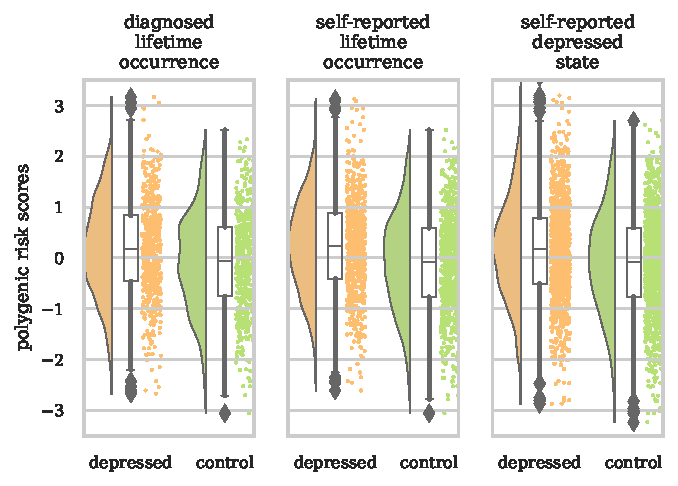
\includegraphics[width=\textwidth]{fig/ukbiobank/PRS_all_analyses_per_cohort_joint}
  \caption{
    UK Biobank depression study distribution of polygenic risk scores for three depression phenotype cohorts.
    Scores are significantly higher for the depressed cohorts compared to the HC cohorts.
  }\label{fig:ukb-lifetime-occurrence-pgs}
\end{figure}


%%
\subsection{Brain regions of interest}
%%

\info[inline]{Paragraph: Frame brain region of interest selection.}
After selecting our cohorts, we need to define and decide on how to characterize brain nodes.
We have opted to study a selection of depression-relevant, anatomically defined brain \glspl{roi}.\improvement{Motivate more why we only look at a selection of brain regions}
We will base this selection on the current understanding of the neurobiology and neurological basis of depression.
Moreover, we pick brain regions that have been the subject of other \gls{fc} studies that looked at the \emph{interaction} between individual brain regions.
The latter will also allow us to validate and contrast our findings within the existing body of work, both \gls{sfc} and \gls{tvfc}.

\info[inline]{Paragraph: Describe brain regions generally involved with depression.}
As reviewed in \cref{sec:fc-depression}, depression is known to primarily affect brain regions involved with mood and reward processing~\parencite{Pandya2012}.
Here we continue this review and motivate in more detail why we study the regions we do.
%
An influential concept in neuroanatomy is that the human brain is in fact made up of three brains.
The concept of this \emph{triune} brain was introduced by \textcite{Maclean1985}.
It posits from an evolutionary perspective that the human brain consists of a primal (`reptilian'; including basal ganglia and brain stem structures that help with the `plumbing' and regulatory side of bodily homeostasis), limbic (`mammalian' or `emotional'; involved with critical emotional skills required for social animals), and neomammalian (`rational'; responsible for higher and more complex cognitive function and regulation of emotions) brain.\footnote{The terms `reptilian' and `mammalian' should, of course, not be taken literally. Reptiles were never ancestors to mammals; our evolutionary lines diverged over 300 million years ago~\parencite{Striedter2019}.}
The primal and limbic systems are more ancient than the (evolutionarily speaking) newer neocortex, and their physiology and anatomy is therefore categorically different as well.
For example, limbic areas such as the \gls{hpc} are typically comprised of three layers, whereas cortical areas typically have five or six layers.
Theories of depression often pertain to such functional descriptions, often suggesting aberrant and dysregulated emotional, limbic, and reward processing~\parencite{Akiskal1973}.
It makes intuitive sense that depression would affect the regions and circuits involved with these functions, as opposed to the visual cortex, for example (although even such regions may very well be affected).
Continuing this tradition, modern computational psychiatry approaches seeking more mechanistic explanations have imposed \gls{rl} concepts such as `utility', `reward', and `value' onto the brain and suggested implementational theories of mood disorders in the human brain~\parencite{Huys2013, Chen2015, Eldar2016, Juechems2019, Bennett2020, Bennett2021}.\footnote{\textbf{Computational psychiatry} broadly refers to computational, model-based approaches to understanding psychiatric illness~\parencite{Montague2012, Adams2016, Radulescu2019, Huys2021}.}
A substantial proportion of the brain is, in fact, involved in processing value functions.
However, key brain regions that have been proposed to be involved in such studies often include the basal ganglia and frontal areas such as the (medial) \gls{ofc}, \gls{vmpfc}, \gls{mpfc}, and (dorsal) \gls{acc}~\parencite{Lee2012}.
%
Yet another source of inspiration comes from applications of the free-energy principle to depression~\parencite{Chekroud2015}.
The idea here is that if the brain does indeed build a generative model of the world, then this will include beliefs about both the external (e.g. intuitive physics) and internal world (e.g. beliefs about agency and helplessness).
Depressive beliefs can then be viewed as those negatively biasing predictions.
Despite these advances, however, it is still unclear what brain regions and networks are exactly involved, and how they may be affected.

\info[inline]{Paragraph: Describe brain regions generally involved with depression (continued).}
The \gls{pfc} has been found to be most consistently impaired with \gls{mdd}~\parencite{George1994, Pizzagalli2021}.
Many subregions of the \gls{pfc} have been individually studied and implicated.
Generally, the \gls{pfc} can be divided into a lateral and a ventromedial part.
Moreover, brain regions related to emotional (e.g.~limbic system constituents) and reward processing are robustly found to be impacted.
Therefore, the brain \glspl{roi} involved with depression that are included in this work are the \gls{amg}~\parencite{Dannlowski2009, Kong2013, Connolly2017, Zhang2020}, \gls{hpc}, \gls{pha}, \gls{ai}~\parencite{Avery2014, Kandilarova2018}, \gls{ofc}~\parencite{Rolls2020}, \gls{pcc}, \gls{dlpfc}, and \gls{acc}~\parencite{Drevets2008} and \gls{mpfc}~\parencite{Pizzagalli2021}.
We will briefly describe what we know about these brain regions before we move on.

The \gls{amg} is an almond-shaped, complex subcortical brain region that is part of the limbic system and is critical in regulating motivation and responses to both rewarding and aversive stimuli~\parencite{Nestler2002}.
It was first described by Karl Friedrich Burdach in 1822~\parencite{Burdach1826}.
It lies in the midbrain, next to the \gls{hpc}, and is connected to many other brain regions.
As a brain structure it is made up of about 13 nuclei.\footnote{In neuroanatomy, a \textbf{nucleus} refers to any cluster of neurons, where such neurons have similar functions and connections to other nuclei.}
The \gls{amg} is especially involved in processing of emotions and memories related to fear, threats, aggression, and pain~\parencite{Thompson2017b}.
It also assigns value and emotional meaning to memories and decisions.
This makes it a prime contestant for relevant brain regions.
It is theorized that the \gls{amg} is dysregulated and hyperactive in patients with \gls{mdd}.
Similarly, the \gls{amg} has been found to be hyperactive in \gls{ptsd} patients, where emotional experiences from memories do not fade over time and keep their original (traumatic) impact.
It has been found that the \gls{amg} has decreased connectivity with a range of other brain regions with \gls{mdd}~\parencite{Tang2013, Ramasubbu2014}.
Even though the \gls{amg} is known to have three functionally distinct subdivisions, we consider it as one whole brain region here.
The \gls{amg} is a relatively small brain region.
\textcite{Brabec2010} found the average \gls{amg} in their sample to be 1,240--1,630~$mm^3$ in size per hemisphere (depending on measurement method, with no significant interhemisphere or intersex differences).
The volume of the \gls{amg} has been shown to shrink with recurrent major depression~\parencite{Sheline1998}.


\begin{figure}[t]
  \centering
  \subcaptionbox{Amygdala (AMG)\label{fig:roi-amg}}{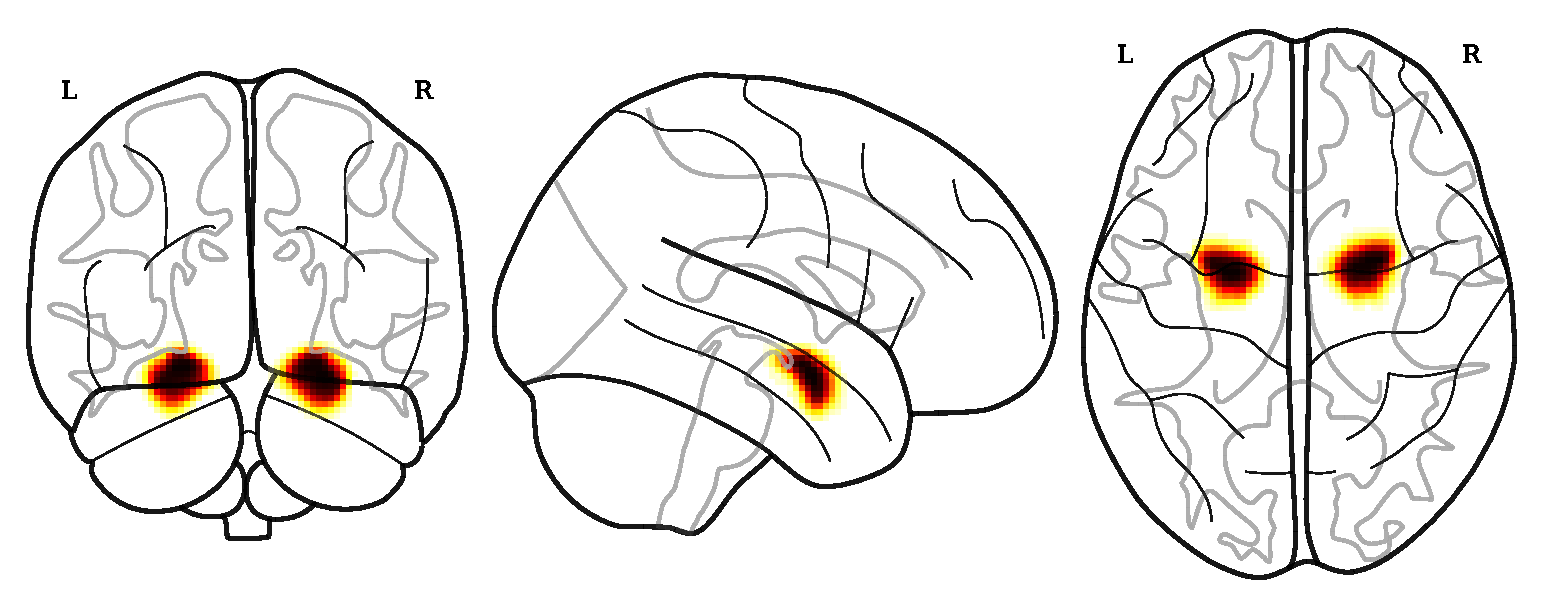
\includegraphics[width=0.37\textwidth]{fig/brain_regions/Amygdala/ho_joint}}
  \hspace{0.08\textwidth}
  \subcaptionbox{Hippocampus (HPC)\label{fig:roi-hpc}}{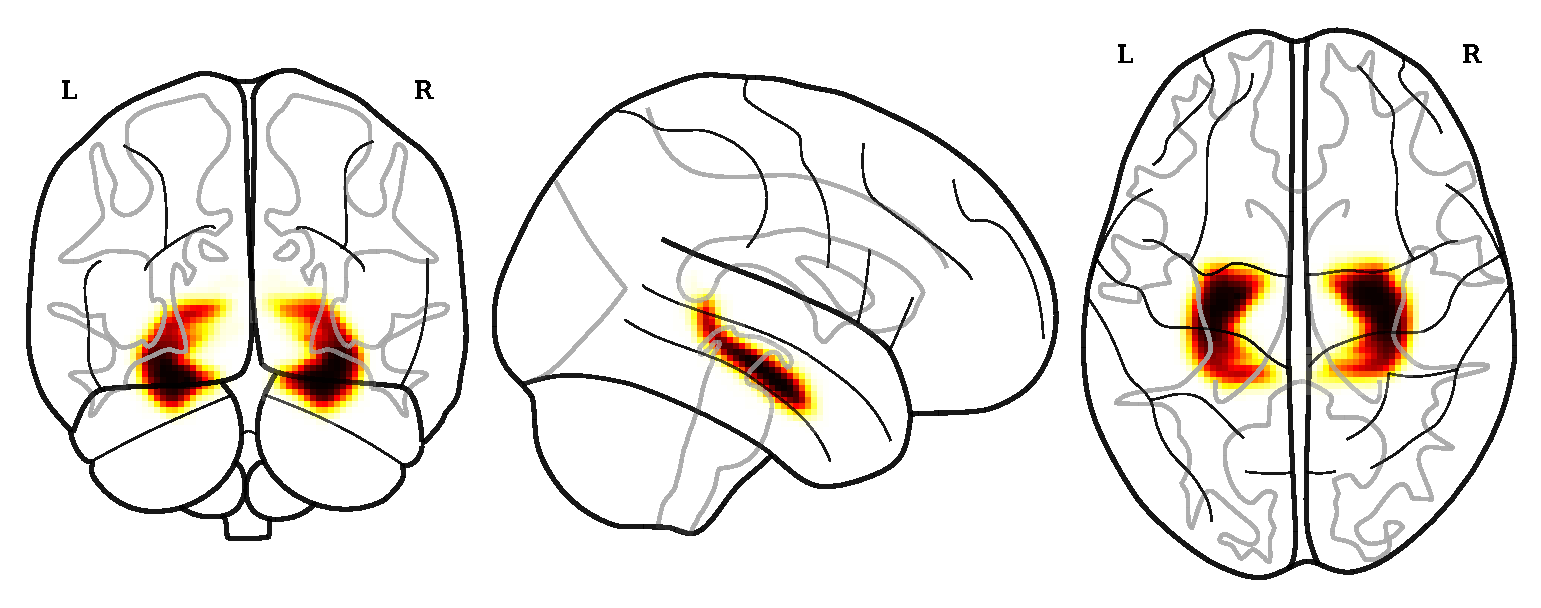
\includegraphics[width=0.37\textwidth]{fig/brain_regions/Hippocampus/ho_joint}}
  \subcaptionbox{Parahippocampal area (PHA)\label{fig:roi-pha}}{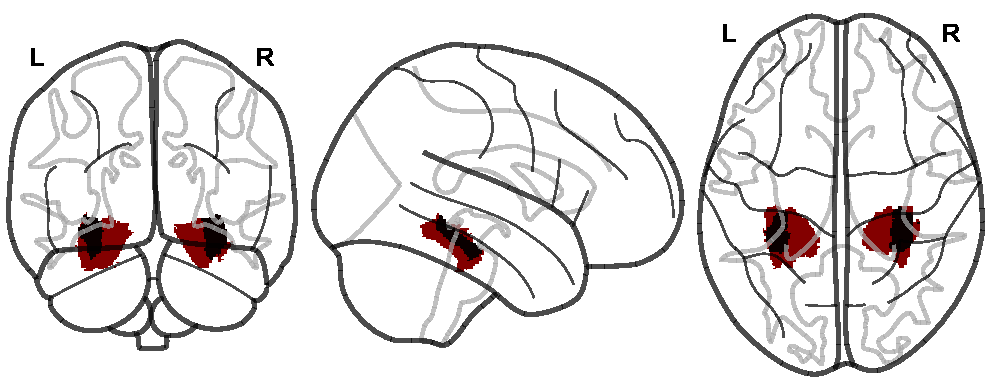
\includegraphics[width=0.37\textwidth]{fig/brain_regions/PHA}}
  \hspace{0.08\textwidth}
  \subcaptionbox{Anterior insula (AI)\label{fig:roi-insula}}{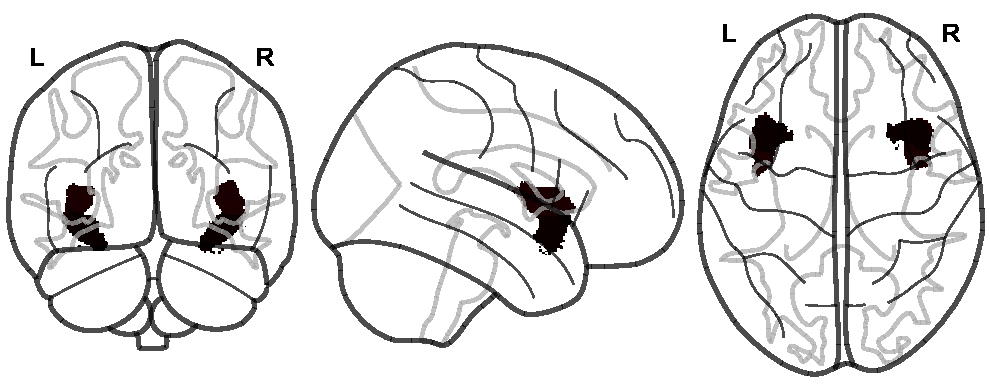
\includegraphics[width=0.37\textwidth]{fig/brain_regions/AI}}
  \subcaptionbox{Orbitofrontal cortex (OFC)\label{fig:roi-ofc}}{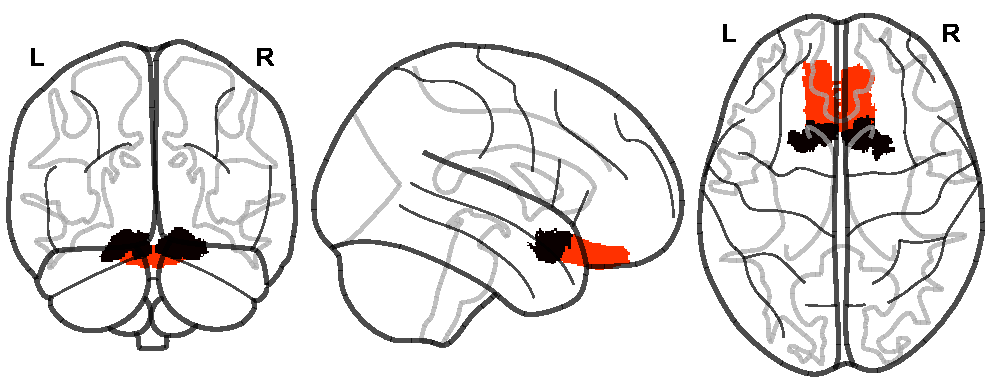
\includegraphics[width=0.37\textwidth]{fig/brain_regions/OFC}}
  \hspace{0.08\textwidth}
  \subcaptionbox{Posterior cingulate cortex (PCC)\label{fig:roi-pcc}}{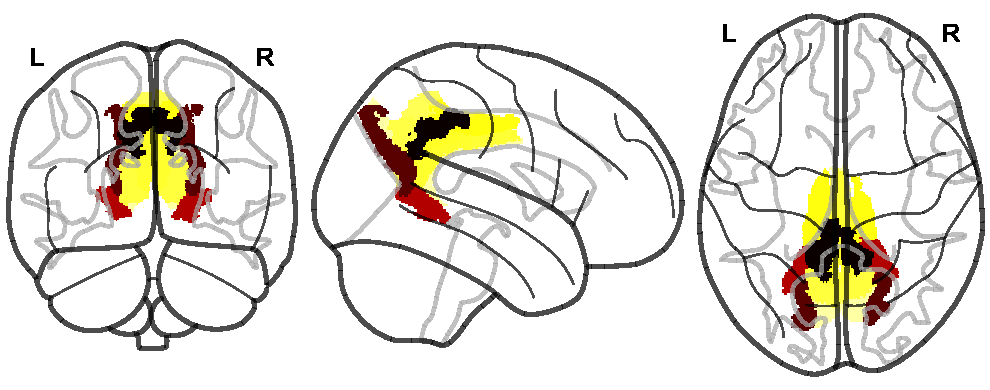
\includegraphics[width=0.37\textwidth]{fig/brain_regions/PCC}}
  \subcaptionbox{Dorsolateral PFC (dlPFC)\label{fig:roi-dlpfc}}{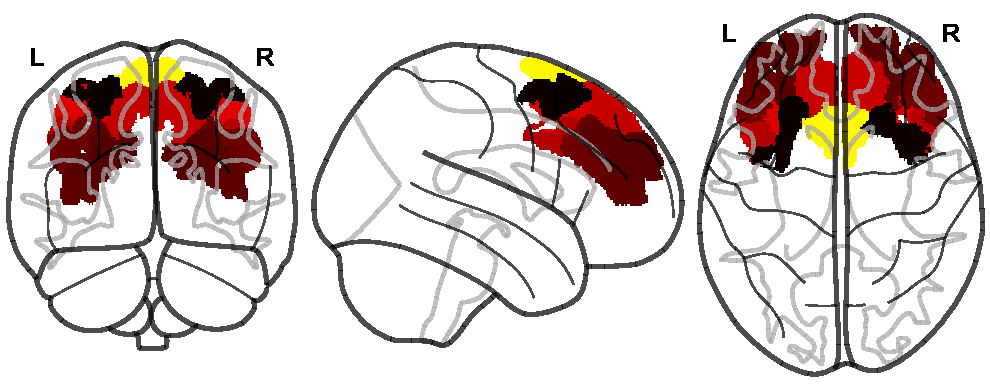
\includegraphics[width=0.37\textwidth]{fig/brain_regions/dlPFC}}
  \hspace{0.08\textwidth}
  \subcaptionbox{Anterior cingulate cortex (ACC)\label{fig:roi-acc}}{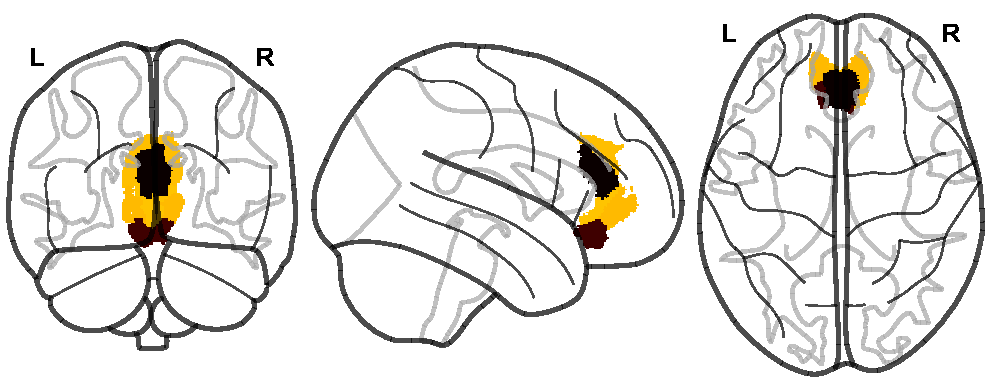
\includegraphics[width=0.37\textwidth]{fig/brain_regions/ACC}}
  \subcaptionbox{Medial PFC (mPFC)\label{fig:roi-mpfc}}{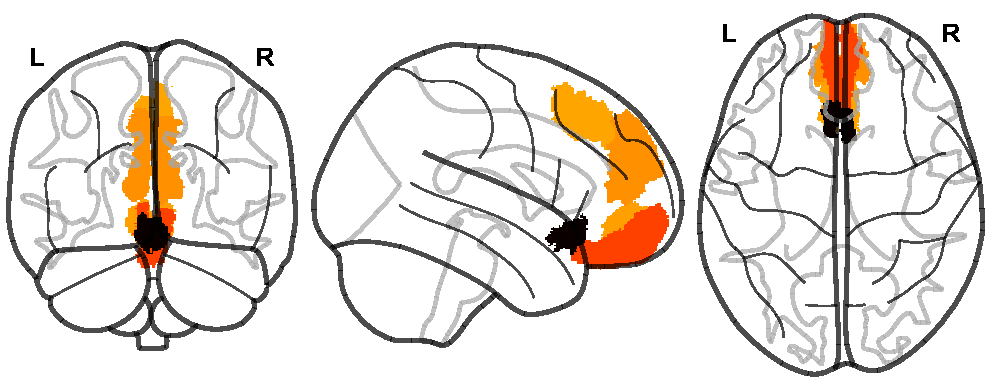
\includegraphics[width=0.37\textwidth]{fig/brain_regions/mPFC}}
  % \hspace{0.08\textwidth}
  % \subcaptionbox{V1 \label{fig:roi-v1}}{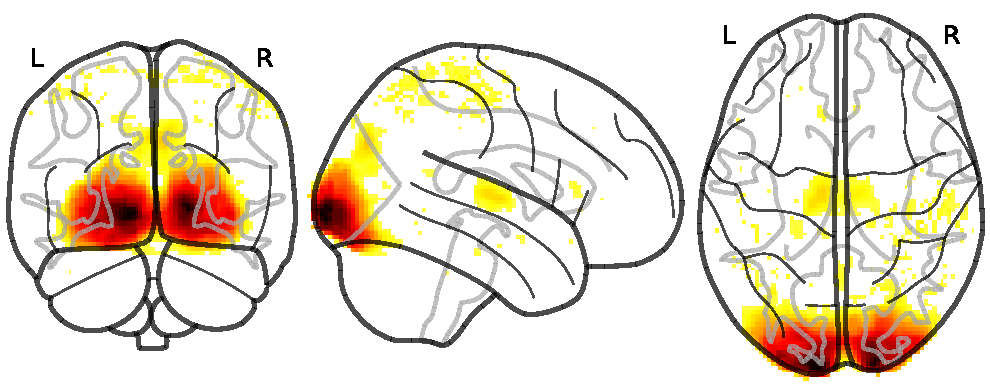
\includegraphics[width=0.38\textwidth]{fig/hcp/RSN_components/RSN_01}}
  \caption{
    Brain ROIs for UK Biobank depression study.
    AMG and HPC are extracted from Harvard-Oxford atlas.
    Other regions are extracted from HCP-MMP1.0 parcellation.
  }\label{fig:ukb-brain-regions}
\end{figure}


The \gls{hpc} is another subcortical region, located deep in the temporal lobe, and is also part of the limbic system.
It has long been known to be involved with learning, memory, and replay of memories (consolidation).
More recently it has also been implied with emotional behavior and spatial navigation.
The \gls{hpc} is a vulnerable brain region, and is one of the earlier and most severely affected brain areas with neurodegenerative disorders such as \gls{ad}.
Hippocampal volumes differ across hemispheres.
\textcite{McHugh2007} found human hippocampal volumes of 3,480~$\pm$~430~$mm^3$ and 3,680~$\pm$~420~$mm^3$ for left and right \gls{hpc}, respectively.
Macaque primate as well as human studies have found decreased hippocampal volume with depression~\parencite{Campbell2004, Malykhin2010, Brown2014, Schmaal2016}.
This is believed to be due to prolonged periods of stress that are often precursors of the onset of depression.
In terms of \gls{fc}, \textcite{Hao2020} found that connectivity between three \gls{hpc} subfields and other brain regions is affected in \gls{mdd}.

The parahippocampus, parahippocampal cortex (PHC), or \gls{pha} is a (grey matter) cortical region that surrounds and is related to the \gls{hpc}~\parencite{Burwell2000}.
It also belongs to the limbic system.
Ramon y Cajal was the one who provided the first and most detailed overview of the (para)hippocampal system.
\textcite{Aminoff2013} proposed that the \gls{pha} processes \emph{contextual associations}.
It becomes more active in \gls{fmri} studies when individuals are shown images of `places' and `situations'~\parencite{Epstein1998}.
\textcite{Megevand2014} showed that stimulation of this region triggered hallucinations of such visuals.
More recent work showed that it also processes \emph{social} context.

The insula, (also known as insular cortex) is part of the \gls{sn} and the limbic system~\parencite{Uddin2017}.
It is known to be involved with modulation of emotional processing.
It has been linked to salience detection, self-awareness, consciousness, interoception, pain processing, and addiction as well~\parencite{Menon2010}.
This is highly related to its function of controlling regulation of the sympathetic and parasympathetic systems.
It also controls awareness of hunger, pain, and fatigue, emotions related to homeostasis that are dysregulated in \gls{mdd}.
Especially the \gls{ai} half is relevant~\parencite{Pasquini2020}, and in this work we only consider this as an \gls{roi}.

The \gls{ofc} is part of the \gls{pfc} and believed to be a nexus for sensory integration.
It is involved with emotional and reward-related behavior~\parencite{Kringelbach2005}.
In a review work, \textcite{Stalnaker2015} finds most evidence for its function in credit and value assignment.
This relates to decision-making as well.

The \gls{pcc}, as part of the cingulate cortex, is located centrally in the brain.
It acts as a central node in the \gls{dmn}.
Functionally, it has many behavioral associations.
As it is linked to daydreaming and memory recollection, in relation to depression it has been linked to rumination.
It has been implied with cognitive control as well~\parencite{Leech2012}.
Overall, its function is still mysterious and may be highly heterogeneous~\parencite{Leech2014}.

The \gls{dlpfc} is part of the lateral \gls{pfc} and is differentiated functionally rather than anatomically.
The \gls{dlpfc} is affected with \gls{mdd} as well, showing lower metabolism~\parencite{Pandya2012}.
This region is mostly linked to executive function (e.g.~planning, reasoning, cognitive flexibility~\parencite{Dajani2015}, and working memory).
It also plays a role in mood regulation.

The \gls{acc} is involved with salience and attention, as well as management of pain and emotions.
It has connections to both the limbic system and prefrontal areas.
Due to its importance in mood regulation, it is one of the most common sites of \gls{dbs} for affective disorders~\parencite{Drevets2008}.
The \gls{acc} is often sub-divided into a rostral or ventral part and a caudal or dorsal part~\parencite[see][for more clarification on subdivisions]{Stevens2011}.

The \gls{mpfc} is another \gls{pfc} subdivision, a part of the ventromedial \gls{pfc}.
It is believed to be involved in introspection (the \gls{mpfc} has one of the highest baseline metabolic rates at rest).
The \gls{mpfc} is another central node in the \gls{dmn} and has been linked to self-referential thought~\parencite{Gusnard2001}.

In our study, only the \gls{bold} time series from these nine brain regions are considered.
All brain regions of interest (as they are implemented in this study) are illustrated in \cref{fig:ukb-brain-regions}.
Interactive three-dimensional brain region plots (in Jupyter Notebooks) are provided upon publication.

\info[inline]{Paragraph: Describe brain region parcellation.}
We use the \gls{hcp} Multi-Modal Parcellation (MMP) 1.0 brain region parcellation~\parencite{Glasser2016}.
This atlas contains 180 regions per hemisphere.
We merge all brain regions across both hemispheres, assuming lateralization does not play a significant role.
Each of the brain regions of interest consists of a collection of subregions from this atlas.
We take a weighted (by number of voxels per subregion) average to obtain our final time series.
Note that parcellation choices are often controversial, see also \textcite{Arslan2018, Bryce2021} for a comparison of parcellation methods.
Subregion specifics (including full names and volumes) are shown in \cref{tab:ukbiobank-brain-regions}.

% The \resizebox scales down the table and its fontsize to \textwidth

\begin{table*}[ht]
  \resizebox{\textwidth}{!}{%
    \begin{tabular}{ l | c | c | c | c }
      \toprule
      \textbf{Macro region}                   & \textbf{Subregion}  & \textbf{Volume ($mm^3$; L/R)} & \textbf{Lobe} & \textbf{Cortex}           \\
      \midrule

      Amygdala (AMG)                          & N/A                 & 1,630 / 1,630                 & Subcortical   & Subcortical               \\

      \midrule

      Hippocampus (HPC)                       & N/A                 & 3,480 / 3,680                 & Subcortical   & Subcortical               \\

      \midrule

      Parahippocampal                         & PHA1                & 1,200 / 1,188                 & Temporal      & Medial temporal           \\
      cortex (PHA)                            & PHA2                & ~~236 / ~~339                 & Temporal      & Medial temporal           \\
                                              & PHA3                & 1,194 / ~~479                 & Temporal      & Medial temporal           \\

      \midrule

      Anterior insula (AI)                    & AAIC                & 1,388 / 1,450                 & Insula        & Insular and frontal opercular   \\
                                              & MI                  & 1,704 / 1,350                 & Insula        & Insular and frontal opercular   \\

      \midrule

      Orbitofrontal                           & OFC                 & 1,834 / 2,105                 & Frontal       & Orbital and polar frontal                 \\
      cortex (OFC)                            & pOFC                & 1,514 / 1,480                 & Frontal       & Anterior cingulate and medial prefrontal  \\

      \midrule

      Posterior cingulate                     & DVT                 & 1,205 / 1,515     & Occipital / Parietal  & Posterior cingulate           \\
      cortex (PCC)                            & ProS                & ~~501 / ~~562     & Parietal              & Posterior cingulate           \\
                                              & POS1                & 1,965 / 2,251     & Parietal              & Posterior cingulate           \\
                                              & POS2                & 2,384 / 2,207     & Occipital / Parietal  & Posterior cingulate    \\
                                              & RSC                 & ~~843 / 1,079     & Parietal              & Posterior cingulate    \\
                                              & v23ab               & ~~690 / ~~702     & Parietal              & Posterior cingulate    \\
                                              & d23ab               & 1,207 / ~~911     & Parietal              & Posterior cingulate    \\
                                              & 31pv                & ~~538 / ~~541     & Parietal              & Posterior cingulate    \\
                                              & 31pd                & ~~586 / ~~307     & Parietal              & Posterior cingulate    \\
                                              & 31a                 & 1,089 / ~~770     & Parietal              & Posterior cingulate    \\
                                              & 23d                 & 1,038 / 1,114     & Parietal              & Posterior cingulate                   \\
                                              & 23c                 & 1,065 / 1,695     & Parietal              & Paracentral lobular and mid cingulate \\
                                              & PCV                 & 1,528 / 1,587     & Parietal              & Posterior cingulate                   \\
                                              & 7m                  & 1,741 / 1,260     & Parietal              & Posterior cingulate                   \\

      \midrule

      Dorsolateral prefrontal                 & 8C                  & 2,982 / 2,734     & Frontal       & Dorsolateral prefrontal       \\
      cortex (dlPFC)                          & 8Av                 & 3,701 / 3,976     & Frontal       & Dorsolateral prefrontal       \\
                                              & i6-8                & 1,357 / 1,798     & Frontal       & Dorsolateral prefrontal       \\
                                              & s6-8                & 1,243 / 1,622     & Frontal       & Dorsolateral prefrontal       \\
                                              & SFL                 & 3,145 / 1,992     & Frontal       & Dorsolateral prefrontal       \\
                                              & 8BL                 & 1,982 / 3,487     & Frontal       & Dorsolateral prefrontal       \\
                                              & 9p                  & 1,693 / 1,419     & Frontal       & Dorsolateral prefrontal       \\
                                              & 9a                  & 3,511 / 2,521     & Frontal       & Dorsolateral prefrontal       \\
                                              & 8Ad                 & 2,508 / 2,036     & Frontal       & Dorsolateral prefrontal       \\
                                              & p9-46v              & 2,655 / 3,311     & Frontal       & Dorsolateral prefrontal       \\
                                              & a9-46v              & 2,738 / 1,890     & Frontal       & Dorsolateral prefrontal       \\
                                              & 46                  & 3,433 / 3,042     & Frontal       & Dorsolateral prefrontal       \\
                                              & 9-46d               & 3,184 / 3,421     & Frontal       & Dorsolateral prefrontal       \\

      \midrule

      Anterior cingulate                      & s32                 & ~~310 / ~~561     & Frontal   & Anterior cingulate and medial prefrontal    \\
      cortex (ACC)                            & p32                 & ~~530 / ~~857     & Frontal   & Anterior cingulate and medial prefrontal    \\
                                              & a24                 & 1,443 / 1,533     & Frontal   & Anterior cingulate and medial prefrontal    \\
                                              & p24                 & 1,427 / 1,403     & Frontal   & Anterior cingulate and medial prefrontal    \\
                                              & d32                 & 1,611 / 1,775     & Frontal   & Anterior cingulate and medial prefrontal    \\

      \midrule

      Medial prefrontal                       & 8BM                 & 2,103 / 2,524     & Frontal   & Anterior cingulate and medial prefrontal    \\
      cortex (mPFC)                           & 9m                  & 4,190 / 4,676     & Frontal   & Anterior cingulate and medial prefrontal    \\
                                              & 10v                 & 2,161 / 2,017     & Frontal   & Anterior cingulate and medial prefrontal    \\
                                              & 10r                 & 1,044 / ~~923     & Frontal   & Anterior cingulate and medial prefrontal    \\
                                              & 25                  & ~~901 / ~~729     & Frontal   & Anterior cingulate and medial prefrontal    \\
      \bottomrule
    \end{tabular}
  }
  \caption{
    UK Biobank macro brain regions of interest subregion constituents.
    Subregions are denoted in HCP-MMP1.0 parcellation nomenclature~\parencite{Glasser2016}.
    Each subregion is further divided in a left- and right hemisphere component.
    % Subregion sizes are denoted in number of voxels.
    % Subregion volume sizes are denoted in $mm^3$.
  }
  \label{tab:ukbiobank-brain-regions}
\end{table*}


An example of extracted node time series for a single subject is shown in \cref{fig:ukb-example-time-series}.


\begin{figure}[t]
  \centering
  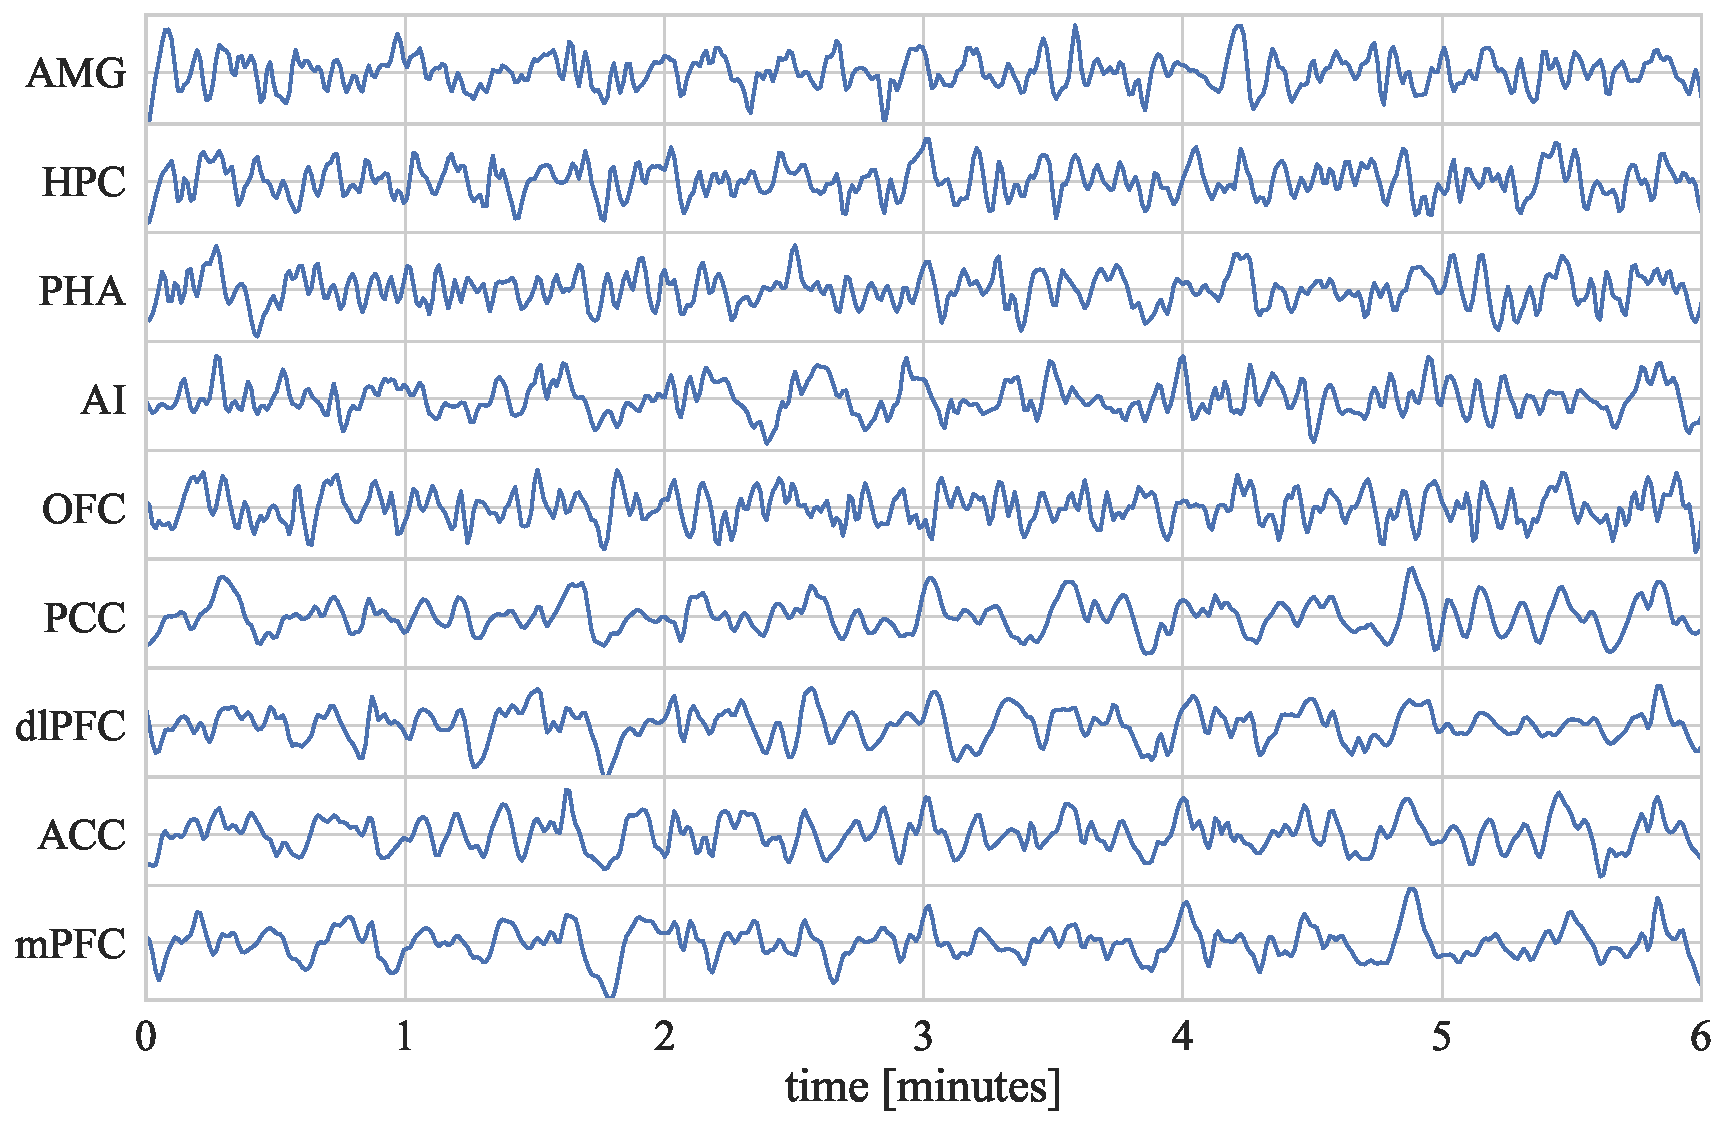
\includegraphics[width=\textwidth]{fig/ukbiobank/node_timeseries/diagnosed_lifetime_occurrence/depressed/time_series_regions_of_interest}
  \caption{
    UK Biobank depression study example time series for all brain regions studied for a single (diagnosed lifetime occurrence, depressed cohort) participant.
  }\label{fig:ukb-example-time-series}
\end{figure}


%%
\subsection{Brain region edges of interest}
%%

\info[inline]{Paragraph: Describe brain region edges of interest decision.}
To limit the scope of our study and to minimize risks related to \gls{mht}, we only look at certain brain region connections (edges).
As with deciding which brain \glspl{roi} to include, from previous findings we also know of several \emph{edges} that are relevant and/or altered with depression.
Especially those previously studied through the lens of \gls{fc} are considered relevant.
The rest of this section reviews such prior work.

However, we must be careful with comparing our results to these prior findings.
The atlases used and brain region definition will be (slightly) different in each experimental setup.
Connectivity measures or interaction indicators vary as well.
Depression phenotypes are typically different across studies.
For example, most studies include participants that were depressed \emph{during} the scan.
Moreover, samples sizes for these studies were often small (see \cref{ch:discussion} for further discussion).

%%
\subsubsection{Static functional connectivity edges affected in depression}
%%

Firstly, we take inspiration from contrasts in \gls{sfc} to understand which edges may be involved.
These will serve as validation as well for the mean of \gls{tvfc} estimates (which should correspond to \gls{sfc} estimates).

Many \gls{amg} to prefrontal areas connectivity disturbances have been reported.
\textcite{Zhang2020} found that \gls{sfc} between the \gls{amg} and \gls{pfc} is \emph{increased} for subjects with \gls{mdd}.
In contrast, \textcite{Dannlowski2009} showed a \emph{decrease} in \gls{fc} between the \gls{amg} and prefrontal areas with \gls{mdd}.
Similarly, \textcite{Kong2013} found decreased \gls{sfc} between the \gls{amg} and left rostral \gls{pfc} with \gls{mdd}.
\textcite{Connolly2017} found reduced \gls{sfc} between the \gls{amg} and both \gls{dlpfc} as well as \gls{vmpfc}.
\textcite{Willinger2022} further showed that prefrontal--\gls{amg} connectivity is affected in adolescents with \gls{mdd}, which they relate to aberrant emotional processing.
\textcite{Burghy2012} found the connection strength of \gls{amg}--\gls{mpfc} to be decreased in those with significant \gls{els}, which (as discussed in \cref{subsec:depression}) is a major confounding factor in developing \gls{mdd}.
\textcite{Rolls2020} found aberrant connectivity between the \gls{amg} and medial \gls{ofc}.
\textcite{Tang2018} also found the \gls{amg} to be involved and its connection to \gls{ofc} changed.

Connectivity between \gls{amg} and other regions has also been studied.
In a seed-based analysis, \textcite{Ramasubbu2014} find decreased \gls{sfc} between the \gls{amg} and many other brain regions, including vlPFC, insula, caudate, precuneus, STG, and occipital regions and \gls{cbm}.
They claim that this reduced connectivity could relate to the dysregulated, hyperactive \gls{amg} in \gls{mdd} patients, and account for a range of depressive symptoms.

\textcite{Rzepa2018} found decreased \gls{sfc} between \gls{dmpfc} and the precuneus.
They also found increased connectivity between the \gls{dmpfc} and \gls{acc}/paracingulate gyrus and with the frontal pole.

Network connectivity changes have also been reported.
The connectivity strength of \gls{pcc}--\gls{mpfc} (key nodes of the \gls{dmn}) was found by \textcite{Philip2013} to be decreased in individuals with \gls{els}.

%%
\subsubsection{Time-varying functional connectivity edges affected in depression}
%%

Although fewer in numbers, there have been several studies that look at straightforward between-group contrasts in \gls{tvfc} summary measures between cohorts.

\textcite{Kaiser2015} found decreased dynamic (less variable) \gls{fc} with depression between \gls{mpfc} and regions of parahippocampal gyrus (i.e.~\gls{pha}) within the default network.
They operationalized \gls{fc} `dynamics' as the standard deviation of estimated \gls{tvfc} using \gls{sw}.
They also found \emph{increased} dynamics between \gls{mpfc} and insula regions, and \gls{mpfc} and \gls{dlpfc}.

\textcite{Demirtas2016} studied `global synchronization' and temporal stability of \gls{fc} in 27 patients and 27 \glspl{hc}.
They find that \gls{sfc} is \emph{increased} within the \gls{dmn} with \gls{mdd}, and \gls{fc} variability \emph{decreased} between \gls{dmn} and \gls{cen}.

\textcite{Wise2017} used a \gls{sw} (40 seconds in length, created using a Gaussian kernel with a standard deviation of 8 seconds) analysis and found increased variance between \gls{pcc} and \gls{mpfc}, the core nodes of the \gls{dmn}.
They linked this finding to correlation with rumination, a core symptom of depression.

\textcite{AlonsoMartinez2020} characterized \gls{fc} dynamics through brain states, and found depressed subjects have overall lower connectivity between \gls{dmn} regions and regions outside of it.
Especially the precuneus was found to be implied.
They also demonstrated how important it is to take the temporal dynamics of \gls{fc} into account.

\textcite{Dini2021} used \gls{sw} and then $k$-means clustering to find three brain states.
They calculated the occupancy rate (OCR), the time that each subject spends in each state.
What they found was that depressed subjects spend less time in a state where connectivity between \gls{cen} and \gls{dmn} was higher than in other states.
\Gls{ect} was seen to increase the amount of time subjects spend in that same state.

\textcite{Ho2021} found lower within-network connectivity (which they refer to as network coherence) in ventral \gls{dmn}, lower within-network connectivity in anterior \gls{dmn} and insula-SN and higher between-network connectivity between \gls{cen} and \gls{dmn}.

As mentioned, it is hard to compare and synchronize these findings, as all of them look at a different way of describing \gls{tvfc} (see \cref{sec:tvfc-feature-extraction}).
However, we start to see a common pattern in prior findings.
One common interpretation of changes in the \gls{dmn} is to link these to rumination and self-referential thinking~\parencite{Zhou2020}.

%%
\subsubsection{List of edges of interest}
%%

Based on these findings, we study the following 13 edges.
We study the edges between the \gls{amg} and four frontal regions: \gls{ofc}, \gls{dlpfc}, \gls{acc}, and \gls{mpfc}.
Two \gls{hpc} edges are studied: those with the \gls{ai} and the \gls{ofc}.
Two \gls{pha} edges are included: those with the \gls{acc} and the \gls{mpfc}.
The edges between the \gls{ai} and the \gls{acc} as well as the \gls{mpfc} are included.  % Kaiser2015
The former of these connections represents \gls{sn} within-network connectivity.
A single \gls{pcc} edge is studied; the one with the \gls{mpfc}.  % Wise2017
This edge represents the \gls{dmn} within-network connectivity.
Finally, we include two more \gls{dlpfc} edges: those with the \gls{acc} and the \gls{mpfc}. % Kaiser2015

%%
\subsection{Functional network analysis}\label{subsec:ukb-fn-analysis}
%%

\info[inline]{Paragraph: Introduce functional networks analysis.}
In our second analysis type, we study brain \emph{networks} instead of individual brain \glspl{roi}.
As reviewed in \cref{subsec:fc-depression}, depression has also been considered as a network disorder.
%
The three networks considered (and described in more detail in \cref{subsec:fc-depression}) in this study are visualized in \cref{fig:ukb-brain-functional-networks}.
The regions and respective sub-regions of these networks are shown in \cref{tab:ukbiobank-functional-networks}.
Which sub-regions (nodes) constitute each specific \gls{fn} is based on \textcite{Fan2016, Uddin2019, Oane2020}.\footnote{There are diverging views on this topic, and we have made an effort to balance out these views.}
Note that IFJa and IFJp could also be part of the middle frontal gyrus instead of the inferior frontal gyrus.
However, we want to make sure there is no overlap between these networks.


\begin{figure}[t]
  \centering
  \subcaptionbox{Central executive network (CEN)\label{fig:fn-cen}}{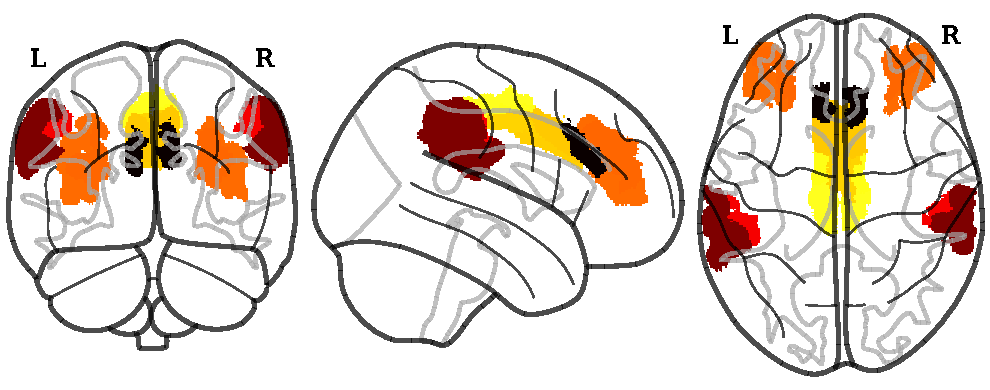
\includegraphics[width=0.50\textwidth]{fig/functional_networks/CEN}}
  \subcaptionbox{Default mode network (DMN)\label{fig:fn-dmn}}{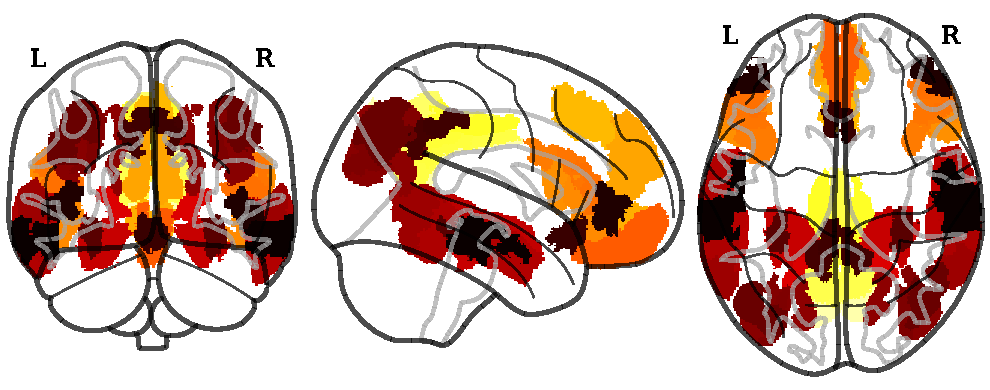
\includegraphics[width=0.50\textwidth]{fig/functional_networks/DMN}}
  \subcaptionbox{Salience network (SN)\label{fig:fn-sn}}{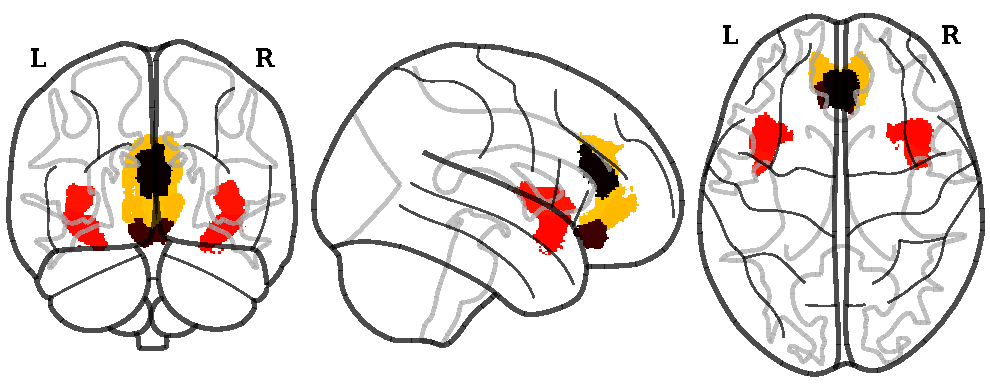
\includegraphics[width=0.50\textwidth]{fig/functional_networks/SN}}
  \caption{
    UK Biobank depression study brain functional networks studied.
    Network subregions are extracted from HCP-MMP1.0 parcellation.
  }\label{fig:ukb-brain-functional-networks}
\end{figure}


% The \resizebox scales down the table and its fontsize to \textwidth

\begin{table*}[t]
  \resizebox{\textwidth}{!}{%
    \begin{tabular}{ l | l | c | c | c | c }
      \toprule
      \textbf{Functional network}     & \textbf{Macro region}           & \textbf{Subregion}    & \textbf{Volume ($mm^3$; L/R)}     & \textbf{Lobe} & \textbf{Cortex}                       \\
      \midrule
      Central executive               & Middle frontal gyrus            & 9-46d                 & 3,184 / 3,421         & Frontal               & Dorsolateral prefrontal                   \\
      network (CEN)                   &                                 & 46                    & 3,433 / 3,042         & Frontal               & Dorsolateral prefrontal                   \\
                                      &                                 & a9-46v                & 2,738 / 1,890         & Frontal               & Dorsolateral prefrontal                   \\
                                      \cmidrule{2-6}
                                      & Anterior inferior               & PFop                  & 1,284 / 1,424         & Parietal              & Inferior parietal                         \\
                                      & parietal lobule                 & PF                    & 4,068 / 3,282         & Parietal              & Inferior parietal                         \\
                                      &                                 & PFt                   & ~~958 / 1,347         & Parietal              & Inferior parietal                         \\
                                      \cmidrule{2-6}
                                      & Midcingulate gyrus              & p24pr                 & 1,039 / 1,336         & Frontal               & Anterior cingulate and medial prefrontal  \\
                                      &                                 & 24dv                  & ~~732 / 1,117         & Frontal               & Paracentral lobular and mid cingulate     \\
                                      &                                 & 24dd                  & 2,287 / 2,279         & Frontal               & Paracentral lobular and mid cingulate     \\
                                      &                                 & 33pr                  & ~~287 / ~~581         & Frontal               & Anterior cingulate and medial prefrontal  \\
                                      &                                 & a24pr                 & ~~854 / ~~938         & Frontal               & Anterior cingulate and medial prefrontal  \\
                                      &                                 & a32pr                 & 1,617 / ~~827         & Frontal               & Anterior cingulate and medial prefrontal  \\
                                      &                                 & p32pr                 & ~~924 / 1,182         & Frontal               & Anterior cingulate and medial prefrontal  \\
      \midrule
      Default mode                    & Medial prefrontal               & 8BM                   & 2,103 / 2,524         & Frontal               & Anterior cingulate and medial prefrontal  \\
      network (DMN)                   & cortex (mPFC)                   & 9m                    & 4,190 / 4,676         & Frontal               & Anterior cingulate and medial prefrontal  \\
                                      &                                 & 10v                   & 2,161 / 2,017         & Frontal               & Anterior cingulate and medial prefrontal  \\
                                      &                                 & 10r                   & 1,044 / ~~923         & Frontal               & Anterior cingulate and medial prefrontal  \\
                                      &                                 & 25                    & ~~901 / ~~729         & Frontal               & Anterior cingulate and medial prefrontal  \\
                                      \cmidrule{2-6}
                                      & Posterior cingulate             & DVT                   & 1,205 / 1,515         & Occipital / Parietal  & Posterior cingulate                       \\
                                      & cortex (PCC)                    & ProS                  & ~~501 / ~~562         & Parietal              & Posterior cingulate                       \\
                                      &                                 & POS1                  & 1,965 / 2,251         & Parietal              & Posterior cingulate                       \\
                                      &                                 & POS2                  & 2,384 / 2,207         & Occipital / Parietal  & Posterior cingulate                       \\
                                      &                                 & RSC                   & ~~843 / 1,079         & Parietal              & Posterior cingulate                       \\
                                      &                                 & v23ab                 & ~~690 / ~~702         & Parietal              & Posterior cingulate                       \\
                                      &                                 & d23ab                 & 1,207 / ~~911         & Parietal              & Posterior cingulate                       \\
                                      &                                 & 31pv                  & ~~538 / ~~541         & Parietal              & Posterior cingulate                       \\
                                      &                                 & 31pd                  & ~~586 / ~~307         & Parietal              & Posterior cingulate                       \\
                                      &                                 & 31a                   & 1,089 / ~~770         & Parietal              & Posterior cingulate                       \\
                                      &                                 & 23d                   & 1,038 / 1,114         & Parietal              & Posterior cingulate                       \\
                                      &                                 & 23c                   & 1,065 / 1,695         & Parietal              & Paracentral lobular and mid cingulate     \\
                                      &                                 & PCV                   & 1,528 / 1,587         & Parietal              & Posterior cingulate                       \\
                                      &                                 & 7m                    & 1,741 / 1,260         & Parietal              & Posterior cingulate                       \\
                                      \cmidrule{2-6}
                                      & Posterior inferior              & PGp                   & 1,808 / 2,911         & Occipital / Parietal  & Inferior parietal                         \\
                                      & parietal lobule                 & PGs                   & 3,143 / 1,902         & Parietal              & Inferior parietal                         \\
                                      &                                 & IP0                   & ~~872 / ~~984         & Occipital / Parietal  & Inferior parietal                         \\
                                      &                                 & IP1                   & 1,154 / 1,194         & Parietal              & Inferior parietal                         \\
                                      \cmidrule{2-6}
                                      & Inferior frontal gyrus          & 44                    & 1,947 / 2,681         & Frontal               & Inferior frontal                          \\
                                      &                                 & 45                    & 2,727 / 2,066         & Frontal               & Inferior frontal                          \\
                                      &                                 & IFJp                  & ~~672 / ~~397         & Frontal               & Inferior frontal                          \\
                                      &                                 & IFJa                  & 1,012 / ~~523         & Frontal               & Inferior frontal                          \\
                                      &                                 & IFSp                  & 1,073 / 1,389         & Frontal               & Inferior frontal                          \\
                                      &                                 & IFSa                  & 1,558 / 1,954         & Frontal               & Inferior frontal                          \\
                                      &                                 & 47l                   & 1,936 / 1,725         & Frontal               & Inferior frontal                          \\
                                      &                                 & p47r                  & 1,330 / 1,577         & Frontal               & Inferior frontal                          \\
                                      \cmidrule{2-6}
                                      & Middle temporal gyrus           & TE1a                  & 4,040 / 3,409         & Temporal              & Lateral temporal                          \\
                                      &                                 & TE1m                  & 2,631 / 2,592         & Temporal              & Lateral temporal                          \\
                                      &                                 & TE1p                  & 5,111 / 4,107         & Temporal              & Lateral temporal                          \\
                                      &                                 & PHT                   & 2,843 / 3,265         & Temporal              & Lateral temporal                          \\
                                      \cmidrule{2-6}
                                      & Parahippocampal cortex          & PHA1                  & 1,200 / 1,188         & Temporal              & Medial temporal                           \\
                                      &                                 & PHA2                  & ~~236 / ~~339         & Temporal              & Medial temporal                           \\
                                      &                                 & PHA3                  & 1,194 / ~~479         & Temporal              & Medial temporal                           \\
                                      \cmidrule{2-6}
                                      & Superior temporal sulcus        & STSda                 & 1,424 / 1,719         & Temporal              & Auditory association                      \\
                                      &                                 & STSdp                 & 1,130 / 1,498         & Temporal              & Auditory association                      \\
                                      &                                 & STSva                 & 1,004 / 1,720         & Temporal              & Auditory association                      \\
                                      &                                 & STSvp                 & 1,644 / 1,985         & Temporal              & Auditory association                      \\
      \midrule
      Salience network (SN)           & Anterior insula (AI)            & AAIC                  & 1,388 / 1,450         & Insula                & Insular and frontal opercular             \\
                                      &                                 & MI                    & 1,704 / 1,350         & Insula                & Insular and frontal opercular             \\
                                      \cmidrule{2-6}
                                      & Anterior cingulate              & s32                   & ~~310 / ~~561         & Frontal               & Anterior cingulate and medial prefrontal  \\
                                      & cortex (ACC)                    & p32                   & ~~530 / ~~857         & Frontal               & Anterior cingulate and medial prefrontal  \\
                                      &                                 & a24                   & 1,443 / 1,533         & Frontal               & Anterior cingulate and medial prefrontal  \\
                                      &                                 & p24                   & 1,427 / 1,403         & Frontal               & Anterior cingulate and medial prefrontal  \\
                                      &                                 & d32                   & 1,611 / 1,775         & Frontal               & Anterior cingulate and medial prefrontal  \\
      \bottomrule
    \end{tabular}
  }
  \caption{
    UK Biobank functional network macro regions and respective subregion constituents.
    Subregions are denoted in HCP-MMP1.0 parcellation nomenclature~\parencite{Glasser2016}.
    Each subregion is further divided in a left- and right hemisphere component.
    % Subregion sizes are denoted in number of voxels.
    % Subregion sizes are denoted in $mm^3$.
  }
  \label{tab:ukbiobank-functional-networks}
\end{table*}


An example of extracted node time series for a single subject is shown in \cref{fig:ukb-fn-example-time-series}.


\begin{figure}[ht]
  \centering
  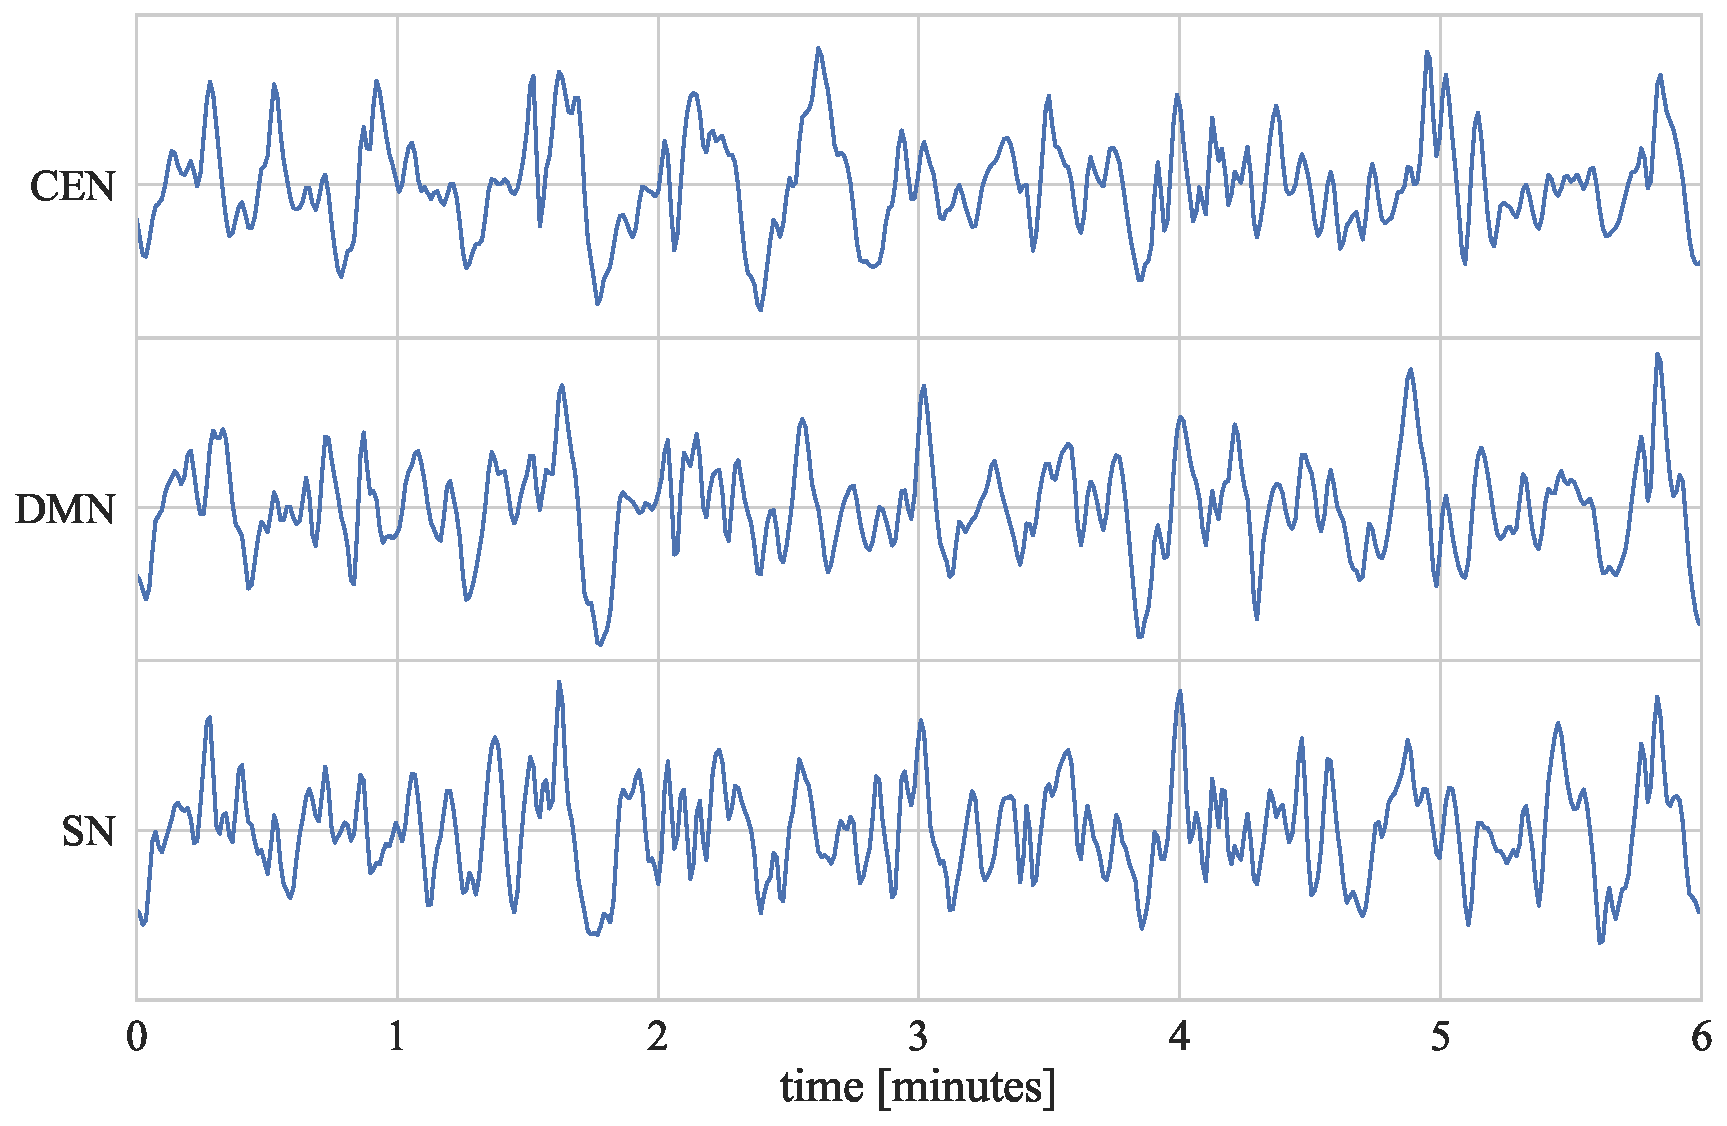
\includegraphics[width=0.8\textwidth]{fig/ukbiobank/node_timeseries/diagnosed_lifetime_occurrence/depressed/time_series_functional_networks_of_interest}
  \caption{
    UK Biobank depression study example time series for all three functional networks studied for a single (diagnosed lifetime occurrence, depressed cohort) participant.
  }\label{fig:ukb-fn-example-time-series}
\end{figure}


In our analysis we look at both within-network connectivity and between-network connectivity.

%%
\subsubsection{Within-network connectivity}
%%

For the \gls{dmn}, within-network connectivity can be defined as connectivity between \gls{mpfc} (i.e.~`posterior \gls{dmn}') and \gls{pcc} (i.e.~`anterior \gls{dmn}'), its two major constituents.
In a large sample study, \textcite{Yan2019} found decreased \gls{sfc} within \gls{dmn}.
They also looked at within and between network connectivity for six other functional networks.
In their review, \textcite{Mulders2015} found that consistent and robust findings from the \gls{sfc} literature include ``increased connectivity within the anterior default mode network'' and ``changed connectivity between the anterior and posterior \gls{dmn}''.

For the \gls{sn}, within-network connectivity can be defined as connectivity between \gls{ai} and (dorsal) \gls{acc}, the two main constituents of this network.

%%
\subsubsection{Between-network connectivity}
%%

We extract characteristic node time series per network ($D = 3$) as a weighted (by subregion size) average of all subregion time series within each functional network.
The detailed subregions included in each \gls{fn} are shown in \cref{tab:ukbiobank-functional-networks}.
Between-network connectivity is then defined as the interaction between these \gls{fn} node time series.

In their review, \textcite{Mulders2015} found that consistent and robust \gls{sfc} findings include ``increased connectivity between the \gls{sn} and the anterior \gls{dmn}'' and ``decreased connectivity between the posterior \gls{dmn} and the \gls{cen}''.
